\section{Grundlagen}

	\subsection{Eingabegeräte für Schwerstmehrfachbehinderte}
    \label{sec:input-devices}
    
    	Aufgrund der Vielzahl an möglichen Behinderungen und Einschränkungen gibt es eine mindestens genau so große Zahl an Eingabemethoden und Geräten. Diese Eingabegeräte können sowohl eine Schnitstelle zu klassischen PCs darstellen oder auch zur Bedienung von unterstützenden Technologien wie z. B. eines Rollstuhls benutzt werden. Im Folgenden sollen hier exemplarisch einige solcher Eingabegeräte vorgestellt werden. Die hier vorgestellte Auswahl ist nicht vollständig und ist aus den Onlinekatalogen der \emph{RehaMedia GmbH}, und der \emph{REHAVISTA GmbH} sowie den Webseiten der erwähnten Hersteller zusammengetragen.
        
        \subsubsection*{Augensteuerung}
        	Bei der Augensteuerung werden mit Hilfe einer Kamera die Bewegungen der Augen genutzt um ein Gerät zu steuern. Damit können dann auch Windows oder OS X Betriebssysteme mit Hilfe eines On-Screen-Menüs gesteuert werden. Der Anbieter \emph{RehaMedia} bewirbt das System \emph{Tobii PCEye} mit den Worten: \enquote{Die Augensteuerung erfasst die Augenbewegungen und setzt sie präzise in Mausbewegungen um. Dank eines Mauszeigermenüs stehen auch bei der Bedienung mit der Augensteuerung alle Mausfunktionen wie Doppelklick, Rechtsklick usw. zur Verfügung.} \parencite{rehamedia:TobiiPCEyeGo}
            
         \subsubsection*{Taster}
         	In der Regel handelt es sich bei Tastern um einen einzelnen großen runden Knopf (\autoref{fig:bigRed}). Es gibt aber auch andere Ausführungen wie einen Griff, welchen man zusammendrücken kann oder einen befestigten Stab gegen den man Druck ausüben kann. Manche Taster können auch an der Kleidung oder an einer Kopfstütze angebracht werden, so dass eine Bedienung nicht nur mit den Händen sondern auch mit dem Kopf oder durch zusammenschlagen der Knie möglich ist. Pedale zur Bedienung mit den Füßen werden auch angeboten. Die meisten Taster verwenden einen 3,5 mm Klinkenstecker und können damit ein diskretes Signal senden. Der Hersteller \emph{ablenet} bietet z. B. Spielsachen an, die so gesteuert werden können (\autoref{fig:penguinRace}). Andere Eingabegeräte können auch Anschlüsse für diese Taster bereitstellen so das diese kombiniert werden können.  
         	
            \begin{figure}[H]
				\centering
				\begin{subfigure}{.5\textwidth}
  					\centering
  					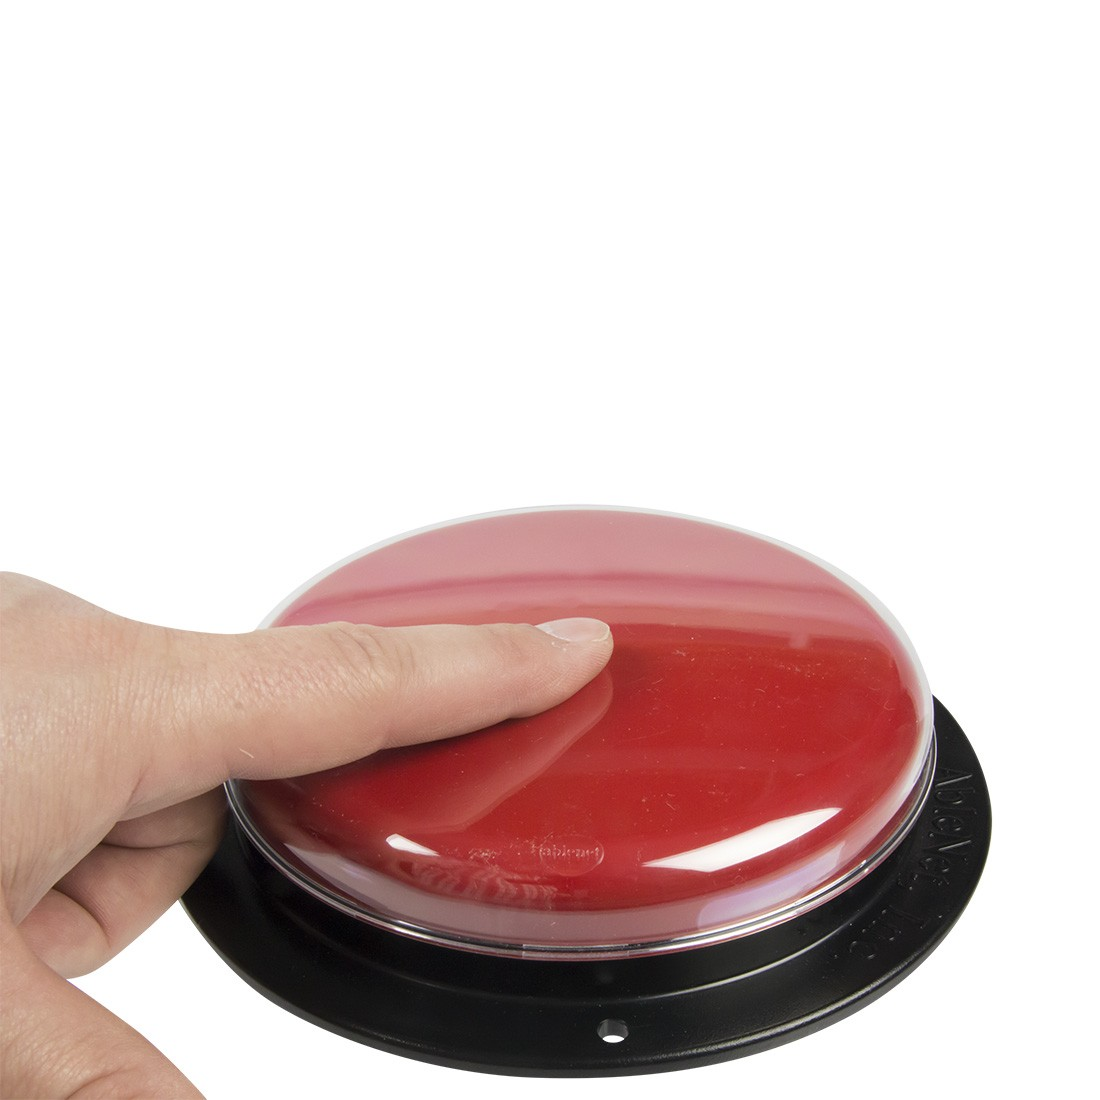
\includegraphics[width=.8\linewidth]{images/big-red-button.jpg}
  					\caption{\emph{Big Red} \cite{ablenet:bigRed}}
                    
  					\label{fig:bigRed}
				\end{subfigure}%
				\begin{subfigure}{.5\textwidth}
  					\centering
  					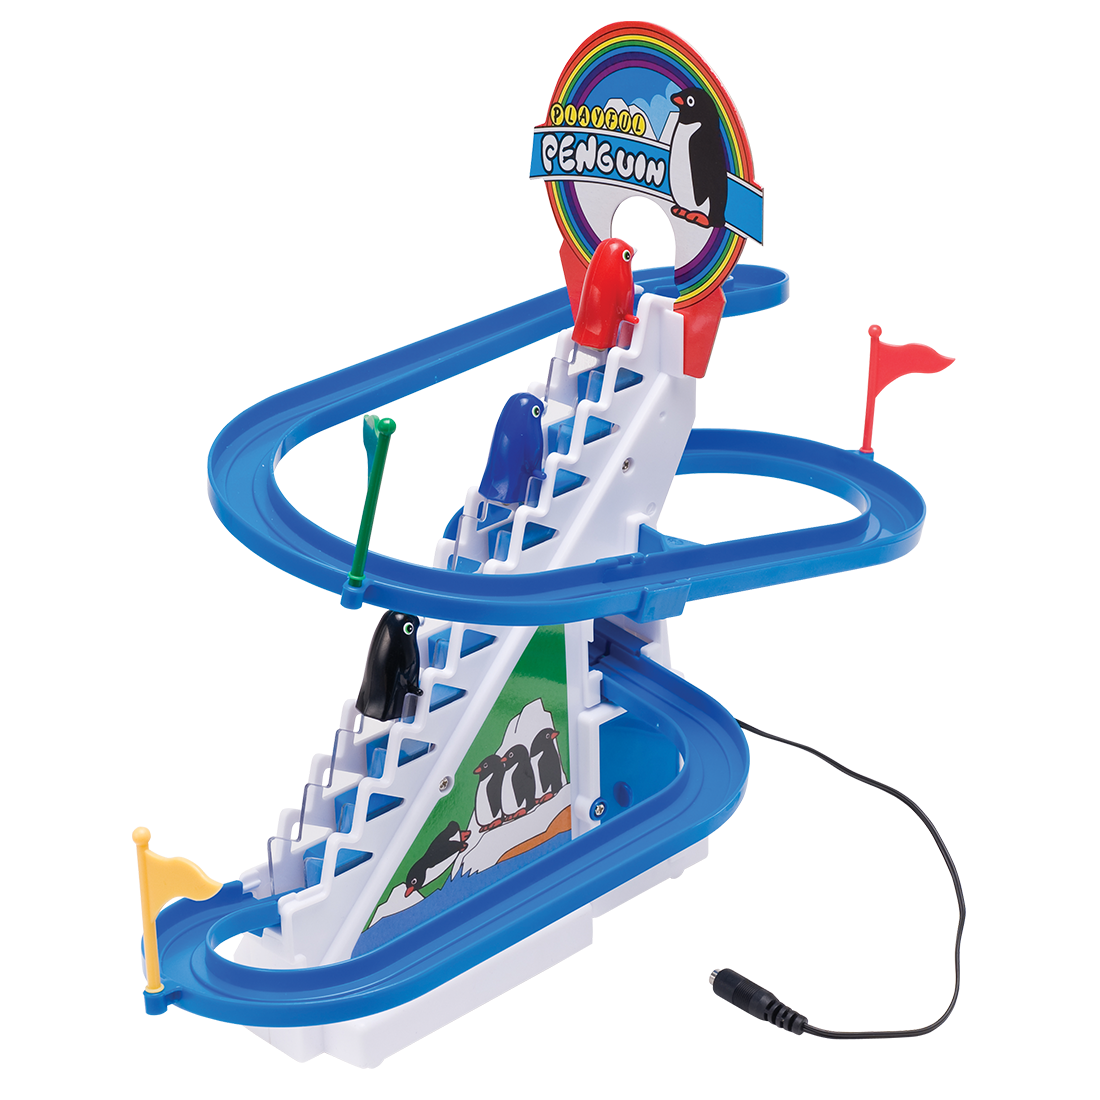
\includegraphics[width=.8\linewidth]{images/penguin-race.png}
  					\caption{\emph{Penguin Race} \cite{ablenet:penguinRace}}
  					\label{fig:penguinRace}
				\end{subfigure}
                \caption{Taster und Spielzeug von ablenet}
				\label{fig:ablenetSingleButtons}
			\end{figure}
            
            Eine weitere Ausführung sind \emph{sprechende Tasten}. Diese Taster haben einen Lautsprecher eingebaut und bieten die Möglichkeit eine oder mehrere Sprachnachrichten aufzunehmen. Wenn mehrere Nachrichten aufgenommen werden können, kann die auszugebende Nachricht von einer betreuenden Person voreingestellt werden. Andere Geräte funktionieren nach dem Prinzip: einmal drücken gibt Nachricht Nummer eins aus, zweimal Nachricht Nummer zwei und dreimal Nachricht Nummer drei.
            
        	Außerdem gibt es Taster mit mehr als einer Taste. Diese sind dann schon zum Anschluss an Computer oder Tablets gedacht und haben häufig einen \emph{USB} oder \emph{Bluetooth} Anschluss. Der Tastenumfang geht dabei von einfachen Geräten mit zwei Tasten bis zu kompletten Computertastaturen.
            
            \begin{figure}[H]
				\centering
				\begin{subfigure}{.33\textwidth}
  					\centering
  					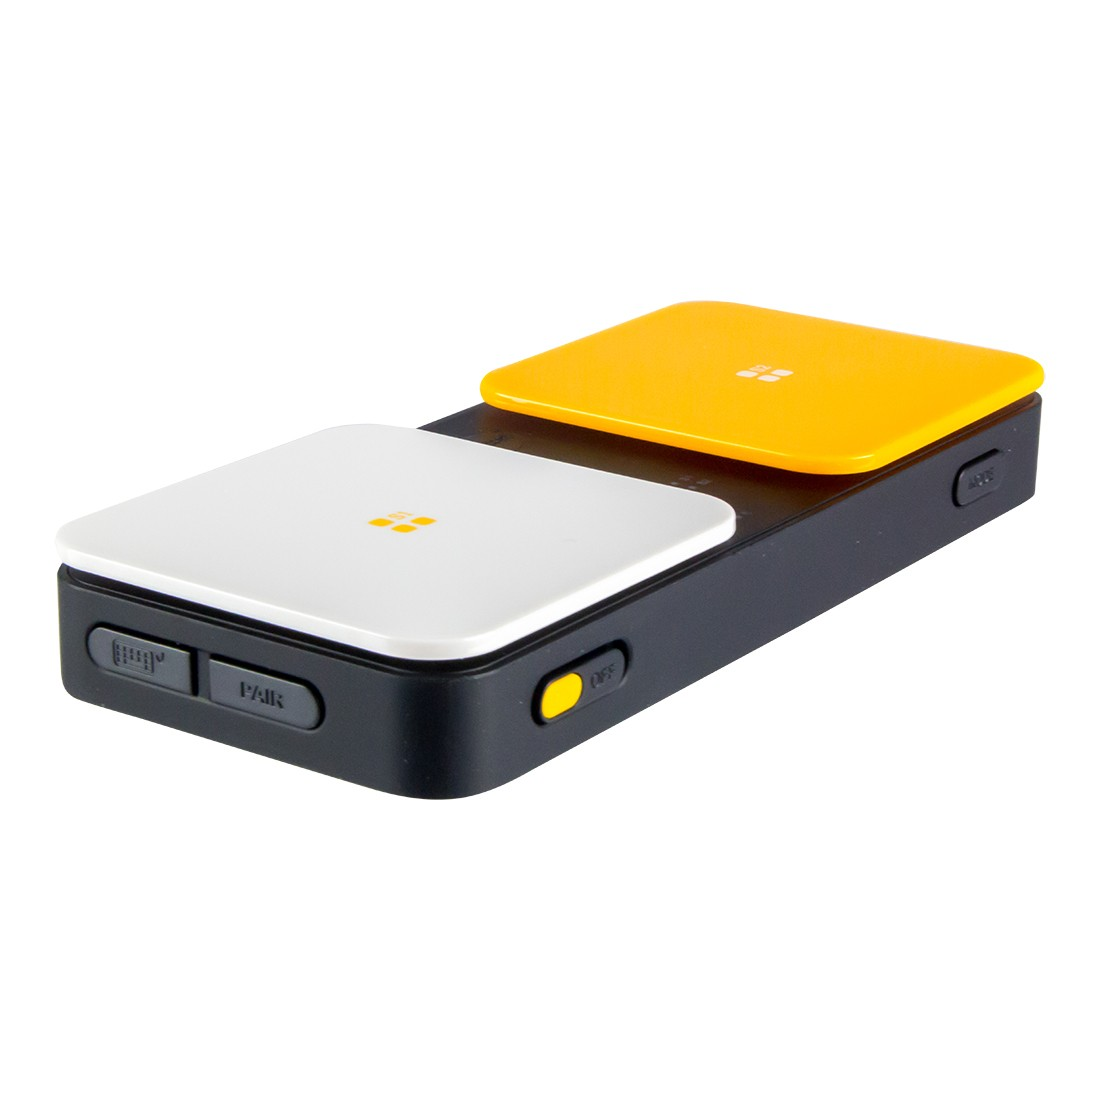
\includegraphics[width=.8\linewidth]{images/buttonsIPad.jpg}
  					\caption{\cite{ablenet:iPad}}
                    
				\end{subfigure}%
				\begin{subfigure}{.33\textwidth}
  					\centering
  					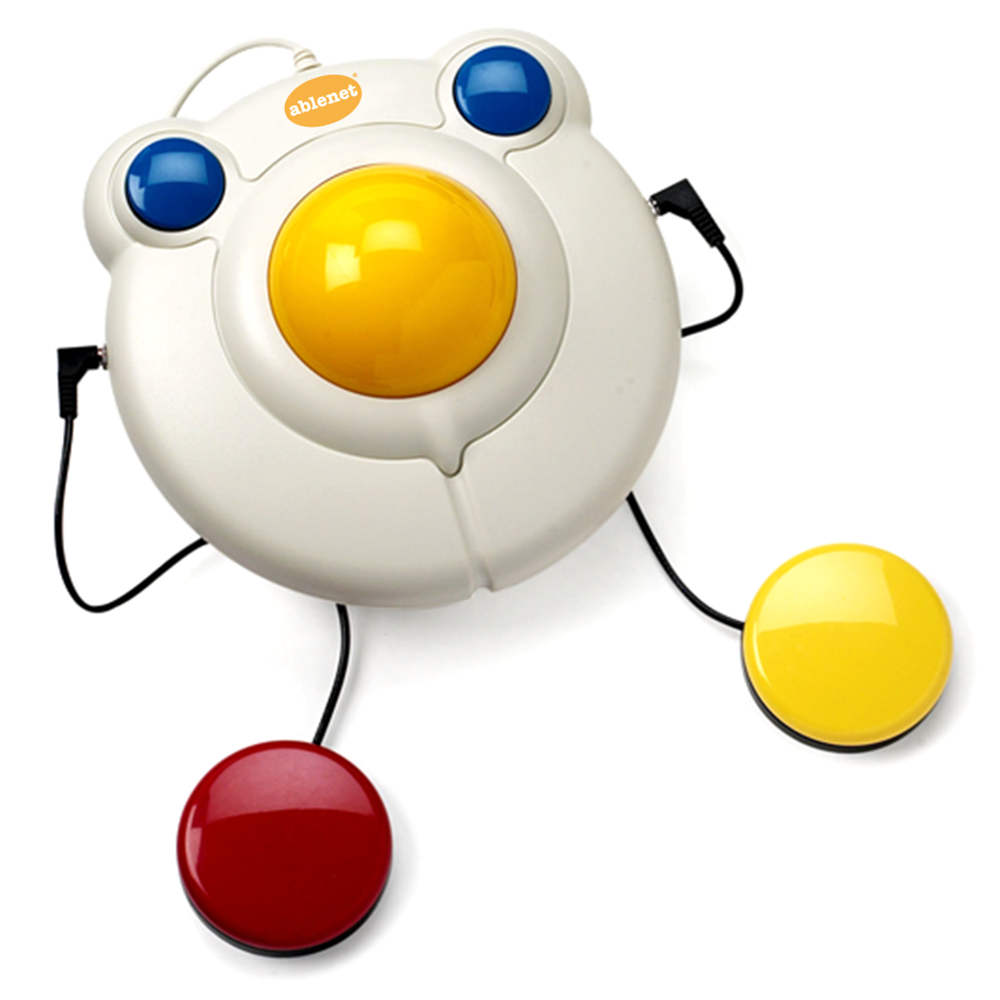
\includegraphics[width=.8\linewidth]{images/buttonsMouse.png}
  					\caption{\cite{ablenet:mouse}}
				\end{subfigure}
                \begin{subfigure}{.33\textwidth}
  					\centering
  					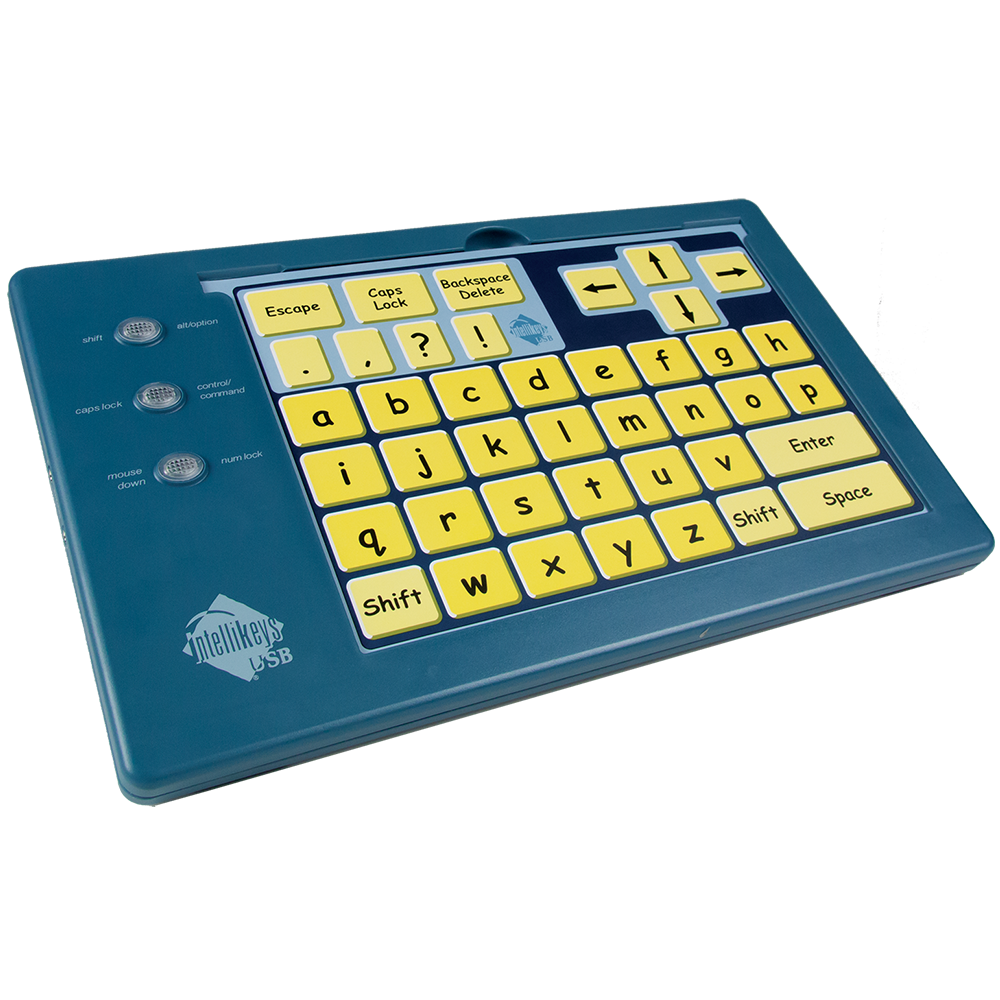
\includegraphics[width=.8\linewidth]{images/buttonsKeyboard.png}
  					\caption{\cite{ablenet:keyboard}}
				\end{subfigure}
                \caption{Taster mit mehreren Tasten von ablenet}
				\label{fig:ablenetMultipleButtons}
			\end{figure}
            
		\subsubsection*{Talker}
        	Bei Talkern handelt es sich um Geräte mit denen durch Knopfdruck Sprache ausgegeben werden kann. Es existieren sowohl statische als auch dynamische Systeme. Bei statischen Systemen sind die Knöpfe fest in der Hardware eingebaut. Dynamische Systeme verwenden Touchscreens. Oft werden dafür auch handelsübliche Tablets mit Schutzhüllen und Halterungen verwendet. 
            
            Diese Systeme können unterschiedlich komplex sein. Einfachere Talker haben ein festes Set an Symbolen welche auf Knopfdruck Sprachnachrichten ausgeben. Dynamische Systeme ermöglichen die Navigation durch verschiedene Symbolgruppen oder arbeiten sogar nur mit Text. Manche ermöglichen auch eine Texteingabe per Tastatur. In \autoref{sec:software-examples} werden verschiedene Softwarelösungen für solche Systeme vorgestellt.
            
            \begin{figure}[H]
				\centering
				\begin{subfigure}{.33\textwidth}
  					\centering
  					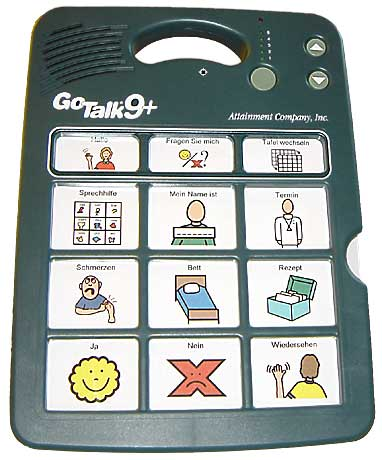
\includegraphics[width=.8\linewidth]{images/goTalkPlus.jpg}
  					\caption{statischer Talker \parencite{rehavista:goTalkPlus}}
                    
				\end{subfigure}%
				\begin{subfigure}{.33\textwidth}
  					\centering
  					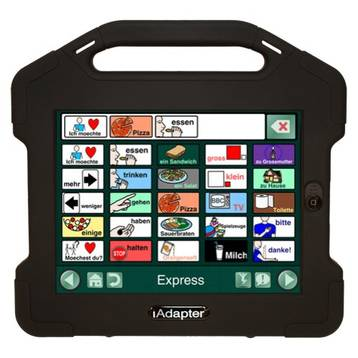
\includegraphics[width=.8\linewidth]{images/goTalkNow.jpg}
  					\caption{iPad mit Talker Erweiterung \parencite{rehamedia:goTalkNow}}
				\end{subfigure}
                \begin{subfigure}{.33\textwidth}
  					\centering
  					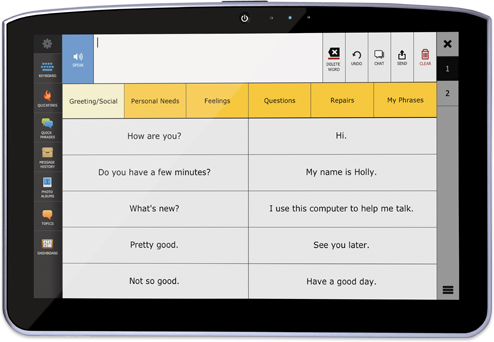
\includegraphics[width=.8\linewidth]{images/tobiiT15.png}
  					\caption{Talker mit literarischem Interface \parencite{tobii:T15}}
				\end{subfigure}
                \caption{verschiedene Talker}
				\label{fig:talker}
			\end{figure}
            
    \newpage
    
    \subsection{Software für Unterstützte Kommunikation}
    \label{sec:software-examples}
    
    	Unter Sprachsoftware wird hier das komplette System von Benutzeroberfläche über mögliche Autovervollständigungen und Eingabevorschlägen bis zur Sprachausgabe verstanden. Im speziellen soll hier Software vorgestellt werden, die auf den in \autoref{sec:input-devices} beschriebenen Talkern anwendung findet. Die Auswahl der Beispiele richtet sich an ihrer Rleveanz für den zu entwickelnden Prototypen. Software deren Funktion den in \autoref{sec:requirements} formulierten Anforderungen nahe kommt.
        
        \subsubsection*{MetaTalkDE / MetaTalkUS}
        	\emph{MetaTalk} ist eine iPad App von \emph{Cidar Health Care LLC} für Symbolbasierte Unterstützte Kommunikation.
            
            \begin{figure}[H]
				\centering
				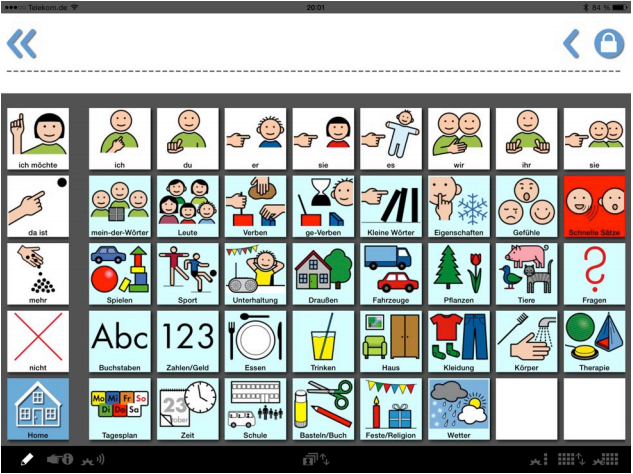
\includegraphics[width=.7\linewidth]{images/Metatalk.png}
                \caption{Schreenshot von MetaTalkDE in der 5x9 Ansicht
                \parencite[p. 8]{cidar:metaTalkManual}}
				\label{fig:metatalk}
			\end{figure}
            
            Auf dem Startbildschirm werden oben in einer Zeile die Ausgewählten Symbole angezeigt. Darunter befindet sich ein Raster mit Symbolen und Kategorien. Durch Auswahl einer Kategorie gelangt man auf einen neuen Bildschirm mit entsprechenden Symbolen.
            Durch druck auf die Symbolzeile oben werden die gelisteten Symbole gesprochen. 
            Die Anzahl der Tasten im Raster ist in drei Stufen (5x9, 4x7, 3x5) anpassbar. Jede Stufe hat auch ein eigenes Vokabular, wobei standartmäsig kleinere Tasten ein größeres Vokabular bedeuten. Die Vokabulare sind innerhalb der App editierbar und können auch über E-Mail exportiert und importiert werden. Die gesammte App bietet viele Möglichkeiten der Personalisierung. So können die Symbole der Tasten ausgetauscht werden, neue Tasten hinzugefügt werden, Tasten mit Farben hinterlegt werden und auch Töne für die Sprachausgabe aufgenommen werden. Nach auswahl von Personalpronomen werden die Verben in der passenden Form angezeigt. Dazu lassen sich durch langes drücken auf ein Symbol andere Formen des entsprechenden Wortes anzeigen. Auch lassen sich \emph{Verlinkungen} erstellen mit denen darauffolgende Symbollisten angeigt werden.
            
            Da die App auf einem iPad läuft muss diese mit den Händen bedient werden. Zwar gibt es die oben beschriebenen \emph{Verlinkungen} jedoch nutzt die App keine Methoden des \emph{Mashine learning} um die Eingabe durch optimierte Symbollisten zu erleichtern.
            
        \subsubsection*{Tobii Sonar Scribe}
    

    
    \subsection{Verwendung von Sprachsoftware im Schulalltag}
    
    Lehrer bereiten Wortschatz für kommende Unterichtstunde vor
    -> funktioiert gut
    -> spontane Unterhaltungen schwierig
    
	\subsection{Sprachsoftware in Unterhaltungs- und Massenelektronik}
    
    \newpage